\documentclass[a4paper,11pt]{article}
\usepackage[T1]{fontenc}
\usepackage[colorlinks=True]{hyperref}
\usepackage[margin=2cm]{geometry}
\usepackage{graphicx}
\usepackage{cleveref}
\setlength\parindent{0pt}
\usepackage{minted}
\usepackage[many]{tcolorbox}
\usemintedstyle{xcode}
\usepackage{xcolor}

\title{Rutherford Scattering Assessment}
\author{Lukasz R Tomaszewski}

\begin{document}

\maketitle

\section{Answers to Questions}

\subsection*{(a)}

The computational problem that this script/ experiment has is in regards to the alpha particles starting location, the x term must be positive while the y terms has to always be negative, if not the plot depicted in \cref{Plot} would not display the incident lines bend away from the gold nucleus, this can be tested and proven by manipulating the [x,y] starting co-ordinates and observe how the output plot pushes the incident lines to the right hand side of the plot thus not representing the Rutherford Scattering experiment properly. In Physics terms, the amount of gold nuclei that is contained within the gold plate could alter the diffraction of the alpha particles path as it penetrates the material and diffracts off. 

\subsection*{(b)}

Even though the simulation in itself is an accurate representation of the Rutherford scattering experiment, thus meaning the values of the parameters can be changed and output the results as if the physical experiment was done separately. In terms of the limitations of the experiment, it cannot contribute the effect of natural forces that are present in the experiment, the simulation has few limitations in regards to this experiment as many parameters such as charge of the gold and alpha particle, speed of light and mass are constants within the simulations and the physical world. 

\subsection*{(c)}

Within the simulation, parameter have been set which are constants within the physical world, the output plot \cref{Plot} shows the physical reaction of the alpha particle diffracting when it comes close to the gold nucleus which when the experiment was completed by Rutherford, shows similarities. Only by changing the parameters could it be seen that the experiment was flawed or mathematically correct, as the simulation is based off the mathematics in bedded into the "Spyder" Python 3.6 script.  

\section{Plot}

\begin{figure}[H]
\centering
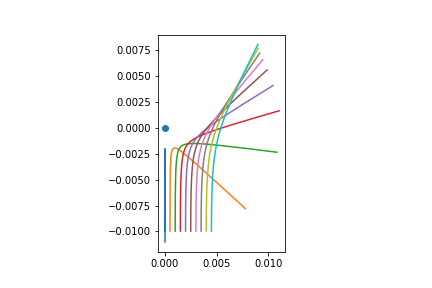
\includegraphics[width=1.0\textwidth]{RSA_Graph.png} 
\caption{Output plot from results of the script} 
\label{Plot}
\end{figure}

\section{Code}

\inputminted[breaklines,linenos]{python3}{RSA.py}
\end{document}